\documentclass[uplatex, dvipdfmx]{jsarticle}
\usepackage{tikz}

\usetikzlibrary{arrows}
\usetikzlibrary{shapes.geometric}
\usetikzlibrary{positioning}
\usetikzlibrary{intersections, calc, arrows}

\begin{document}
  \begin{figure}[ht]
    \centering
    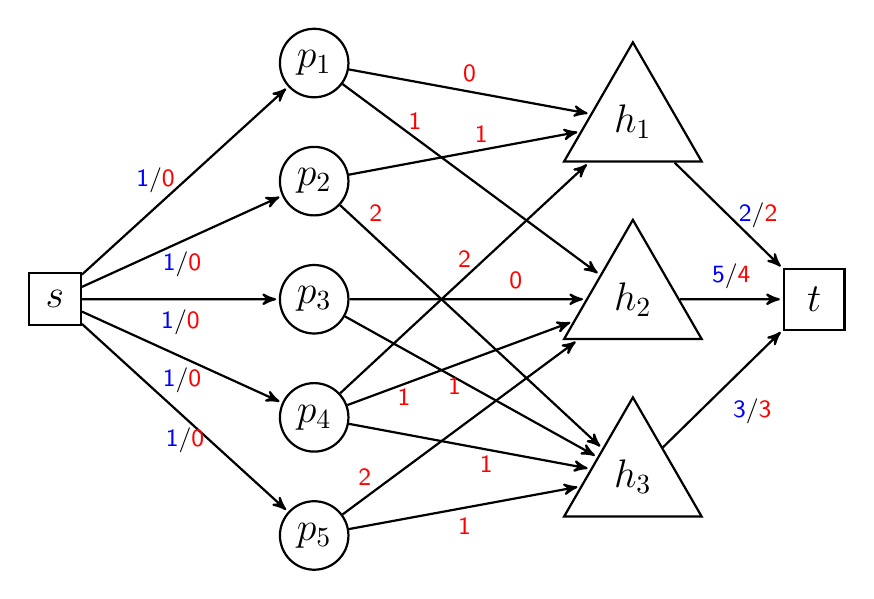
\begin{tikzpicture}[->,>=stealth',shorten >=1pt,auto,node distance=1.5cm,thick,
        square/.style={regular polygon,regular polygon sides=4},
        triangle/.style={regular polygon,regular polygon sides=3},
        pat node/.style={circle,draw,font=\sffamily\Large\bfseries},
        hos node/.style={triangle,draw,font=\sffamily\Large\bfseries},
        ext node/.style={square,draw,font=\sffamily\Large\bfseries}
        ]

        \node[pat node](1){$p_1$};
        \node[pat node](2)[below of=1]{$p_2$};
        \node[pat node](3)[below of=2]{$p_3$};
        \node[pat node](4)[below of=3]{$p_4$};
        \node[pat node](5)[below of=4]{$p_5$};

        \node[hos node](7)[right =3cm of 3]{$h_2$};
        \node[hos node](6)[above=0.7cm of 7]{$h_1$};
        \node[hos node](8)[below=0.7cm of 7]{$h_3$};

        \node[ext node](s)[left=2.5cm of 3]{$s$};
        \node[ext node](t)[right=5.5cm of 3]{$t$};

        \path[every node/.style={font=\sffamily\small}]
        (s) edge node[left]{\textcolor{blue}{1}/\textcolor{red}{0}} (1)
        (s) edge node[below]{\textcolor{blue}{1}/\textcolor{red}{0}} (2)
        (s) edge node[below]{\textcolor{blue}{1}/\textcolor{red}{0}} (3)
        (s) edge node[below]{\textcolor{blue}{1}/\textcolor{red}{0}} (4)
        (s) edge node[below]{\textcolor{blue}{1}/\textcolor{red}{0}} (5)

        (6) edge node[right]{\textcolor{blue}{2}/\textcolor{red}{2}} (t)
        (7) edge node[above]{\textcolor{blue}{5}/\textcolor{red}{4}} (t)
        (8) edge node[below right]{\textcolor{blue}{3}/\textcolor{red}{3}} (t)

        (1) edge node[above]{\textcolor{red}{0}} (6)
        (1) edge node[above left=0.5cm and 0.5cm]{\textcolor{red}{1}} (7)
        (2) edge node[above right]{\textcolor{red}{1}} (6)
        (2) edge node[above left=1.2cm and 1cm]{\textcolor{red}{2}} (8)
        (3) edge node[above right=0.01cm and 0.4cm]{\textcolor{red}{0}} (7)
        (3) edge node[left]{\textcolor{red}{1}} (8)
        (4) edge node[above]{\textcolor{red}{2}} (6)
        (4) edge node[below left=0.2cm and 0.5cm]{\textcolor{red}{1}} (7)
        (4) edge node[below right]{\textcolor{red}{1}} (8)
        (5) edge node[below left=0.4cm and 1cm]{\textcolor{red}{2}} (7)
        (5) edge node[below]{\textcolor{red}{1}} (8);

    \end{tikzpicture}

    \label{fig-1}
    \caption{flow networkの例(各辺のタグは青がcapacity(省略は$1$)、赤がcost)}
\end{figure}
\end{document}
